\documentclass{article}
\usepackage{v-test-paper}
%\renewcommand{\ans}{\quad}
\title{Module-Test-10\\(Physics-NEET)}
\begin{document}

\maketitle

\neetSectionA
\begin{enumerate}
\item For the given graph find the work done by the force.
\begin{center}
\begin{tikzpicture}
	\tzaxes(-0.5, -0.5)(5, 3){$x$}{$F$}
	\tzticks(-1pt:1pt){1/$1$, 2/$2$, 3/$3$, 4/$4$}(-1pt:1pt){1/$1$, 2/$2$}
	\tzlines(0, 0)(2, 2)(4, 0);
	\tzproj[dashed, red](2,2)
\end{tikzpicture}
\end{center}
\begin{tasks}(2)
	\task $8\Joule$
	\task $-8\Joule$
	\task $-4\Joule$
	\task $4\Joule$\ans
\end{tasks}


\item A bucket tied to a string is lowered at a constant acceleration of $g/4$. If mass of the bucket is $m$ and it is lowered by a distance $l$ then find the work done by the string on the bucket.
\begin{tasks}(2)
	\task $-\dfrac{3}{4}mgl$\ans
	\task $\dfrac{3}{4}mgl$
	\task $\dfrac{4}{3}mgl$
	\task $-\dfrac{4}{3}mgl$
\end{tasks}


\item A block is constrained to move along x-axis under a force $F = 10$ acting at an angle of $60^\circ$. Find the work done by this force when the block is displaced from $x = 0 \m$ to $x = 2 \m$.
\begin{center}
\begin{tikzpicture}
\pic {frame=5cm};
\node[block] at (-1, 0.4)(block){};
\tzline+[->](block.east)(1, 1.5){$F=10$}[r]
\tzline+[dashed](block.east)(1.5, 0)
\tzanglemark(2, 0.4)(block.east)(0.8, 2.5){$60^\circ$}(15pt)
\end{tikzpicture}
\end{center}
\begin{tasks}(2)
	\task $-20\Joule$
	\task $10\Joule$\ans
	\task $-10\Joule$
	\task $20\Joule$
\end{tasks}


\item Displacement of a particle of mass $2 \kg$ varies with time as $s = (2t^2 - 2t + 10) \m$. Find total work done on the particle in a time interval from $t = 0$ to $t = 2 \s$.
\begin{tasks}(2)
	\task $-32\Joule$
	\task $16\Joule$
	\task zero
	\task $32\Joule$\ans
\end{tasks}

\item A $5\kg$ mass is raised a distance of $4\m$ by a vertical force of $80\N$. Find the final kinetic energy of the mass if it was originally at rest. $g = 10\mpss$.
\begin{tasks}(2)
	\task $100\Joule$
	\task $-100\Joule$
	\task $120\Joule$\ans
	\task None of these
\end{tasks}

\item Work done when a force $F=(\hat{i}+2\hat{j}+3\hat{k})\N$ acting on a particle takes it from the point $\vec{r}_1 = (\hat{i} + \hat{j} + \hat{k} )$ to the point $\vec{r}_2 = (\hat{i} - \hat{j} + 2 \hat{k} )$ is
\begin{tasks}(2)
	\task $-3\Joule$
	\task $-1\Joule$\ans
	\task zero
	\task $2\Joule$
\end{tasks}


\item A block is constrained to move along x-axis under a force $F = - 2x$ . Here, $F$ is in newton and $x$ in
metre. Find the work done by this force when the block is displaced from $x = 2 \m$ to $x = - 4 \m$.
\begin{center}
\begin{tikzpicture}
\pic {frame=5cm};
\node[block] at (-1, 0.4)(block){};
\tzline+[->](block.east)(1.5, 0){$F$}[r]
\end{tikzpicture}
\end{center}
\begin{tasks}(2)
	\task $12\Joule$
	\task $-12\Joule$\ans
	\task $8\Joule$
	\task $-8\Joule$
\end{tasks}

\item A force $F=(3t\hat{i}+5\hat{j})\N$ acts on a body due to which its displacement varies as $S=(2t^2\hat{i}-5\hat{j})\m$. Work done by this force in $2\s$ is
\begin{tasks}(2)
	\task $32\Joule$\ans
	\task $24\Joule$
	\task $46\Joule$
	\task $20\Joule$
\end{tasks}

\item Under the action of a force, a $2 \kg$ body moves such that its position $x$ as a function of time is given by $x=\dfrac{t^3}{3}$, where $x$ is in metre and $t$ in second. The work done by the force in the first two seconds is
\begin{tasks}(2)
	\task $1600\Joule$
	\task $160\Joule$
	\task $16\Joule$\ans
	\task $1.6\Joule$
\end{tasks}

\item A force $F_1$ accelerates a particle from rest to a velocity $v$. Another force $F_2$ decelerates the same particle from $v$ to rest, then
\begin{tasks}(1)
	\task $F_1$ is always equal to $F_2$\ans
	\task $F_2$ is greater than $F_1$
	\task $F_2$ may be smaller than, greater than or equal to $F_1$
	\task $F_2$ cannot be equal to $F_1$
\end{tasks}


\item A particle is moving on a circular track of radius $30 \cm$ with a constant speed of $6 \mps$. Its acceleration is
\begin{tasks}(2)
	\task zero
	\task $120\mpss$\ans
	\task $1.2\mpss$
	\task $36\mpss$
\end{tasks}

\item In case of a uniform circular motion, velocity and acceleration are
\begin{tasks}(2)
	\task perpendicular\ans
	\task in same direction
	\task in opposite direction
	\task not related to each other
\end{tasks}

\item Force $F$ on a particle moving in a straight line varies with distance $d$ as shown in the figure. The work done on the particle during its displacement of $12\m$ is
\begin{center}
\begin{tikzpicture}[xscale=0.5]
	\tzaxes(-1, -0.5)(14, 3){$d$}{$F$}
	\tzlines(3, 2)(7, 2)(12, 0);
	\tzticks(-1pt:1pt){3/$3$, 7/$7$, 12/$12$}(-1pt:1pt){2/$2$}
	\tzproj[dashed, red](3, 2)
\end{tikzpicture}
\end{center}
\begin{tasks}(2)
	\task $21\Joule$
	\task $26\Joule$
	\task $13\Joule$\ans
	\task $18\Joule$
\end{tasks}

\item The speed of a particle moving in a circle is increasing. The dot product of its acceleration and velocity is
\begin{tasks}(2)
	\task negative
	\task zero
	\task positive\ans
	\task maybe positive or negative
\end{tasks}

\item A car wheel is rotated to uniform angular acceleration about its axis. Initially its angular velocity is zero. It rotates through an angle $\theta_1$ in the first $2 \s$. In the next $2 \s$, it rotates through an additional angle $\theta_2$ , the ratio of $\dfrac{\theta_2}{\theta_1}$ is
\begin{tasks}(2)
	\task $1$
	\task $2$
	\task $3$\ans
	\task $4$
\end{tasks}

\item Two particles of equal masses are revolving in circular paths of radii $r_1$ and $r_2$ respectively with the same speed. The ratio of their centripetal forces is
\begin{tasks}(2)
	\task $\dfrac{r_2}{r_1}$\ans
	\task $\sqrt{\dfrac{r_2}{r_1}}$
	\task $\left(\dfrac{r_1}{r_2}\right)^2$
	\task $\left(\dfrac{r_2}{r_1}\right)^2$
\end{tasks}

\item The maximum tension that an inextensible ring of radius $1\m$ and mass density $0.1 kg \m^{-1}$ can bear is $40 \N$. The maximum angular velocity with which it can be rotated in a circular path is
\begin{tasks}(2)
	\task $20\text{rad}/\s$\ans
	\task $18\text{rad}/\s$
	\task $16\text{rad}/\s$
	\task $15\text{rad}/\s$
\end{tasks}

%bonus
\item Three identical particles are joined together by a thread as shown in figure. All the three particles are moving in a horizontal plane. If the velocity of the outermost particle is $v_0$ , then the ratio of tensions in the three sections of the string is
\begin{center}
\begin{tikzpicture}
\coordinate(O) at (0, 0);
\def\r{2}
	\tzdots*(O){$O$}[b]($(O)+(\r, 0)$){$A$}[b]($(O)+(2*\r, 0)$){$B$}[b]($(O)+(3*\r, 0)$){$C$}[b];(4pt)
	\tzlines(O)($(O)+(\r, 0)$)($(O)+(2*\r, 0)$)($(O)+(3*\r, 0)$);
	\tzline[|<->|]<0, -0.7>(O)($(O)+(\r, 0)$){$l$}[b, midway]
	\tzline[|<->|]<0, -0.7>($(O)+(\r, 0)$)($(O)+(2*\r, 0)$){$l$}[b, midway]
	\tzline[|<->|]<0, -0.7>($(O)+(2*\r, 0)$)($(O)+(3*\r, 0)$){$l$}[b, midway]
\end{tikzpicture}
\end{center}
\begin{tasks}(2)
	\task $3:2:1$\ans
	\task $3:4:5$
	\task $7:11:6$
	\task $3:5:6$
\end{tasks}

\item A national roadway bridge over a canal is in the form of an arc of a circle of radius $49 \m$. What is the maximum speed with which a car can move without leaving the ground at the highest point? (Take $g = 9.8 \mpss$ )
\begin{tasks}(2)
	\task $19.6\mps$
	\task $40\mps$
	\task $22\mps$\ans
	\task None of these
\end{tasks}

\item A force $F$ acting on an object varies with distance $x$ as shown here. The force is in newton and $x$ is in metre. The work done by the force in $x=0$ to $x=6\m$ is
\begin{center}
\begin{tikzpicture}
	\tzaxes(-1, -4)(8, 4){$x$}{$F$}
	\tzlines(0, -3)(3, 0)(6, 3);
	\tzticks(-1pt:1pt){3/$3$, 6/$6$}(-1pt:1pt){-3/$-3$, 3/$3$}
	\tzproj[dashed, red](6, 3)
\end{tikzpicture}
\end{center}
\begin{tasks}(2)
	\task $4.5\Joule$
	\task $0\Joule$\ans
	\task $9.0\Joule$\ans
	\task $18.0\Joule$
\end{tasks}

\item A force $F=20+10y$ acts on a particle in y-direction, where $F$ is in newton and $y$ in meter. Work done by this force to move the particle from $y=0$ to $y=1\m$ is
\begin{tasks}(2)
	\task $5\Joule$
	\task $25\Joule$\ans
	\task $20\Joule$
	\task $30\Joule$
\end{tasks}

\item A particle moves from a point $(-2\hat{i} + 5\hat{j})$ to $(4\hat{j} + 3\hat{k})$ when a force of $(4\hat{i} + 3\hat{j})\N$ is applied. How much work has been done by the force?
\begin{tasks}(2)
	\task $8\Joule$
	\task $11\Joule$
	\task $5\Joule$\ans
	\task $2\Joule$
\end{tasks}

\item A uniform force of $(3\hat{i} + \hat{j})\N$ acts on a particle of mass $2\kg$. Hence, the particle is displaced from position $(2\hat{i}+\hat{k})\m$ to position $(4\hat{i} +3\hat{j} -\hat{k})\m$. The work done by the force on the particle is
\begin{tasks}(2)
	\task $9\Joule$\ans
	\task $6\Joule$
	\task $13\Joule$
	\task $15\Joule$
\end{tasks}



\item A force $F$ acting on an object varies with distance $x$ as shown here. The force is in newton and $x$ is in metre. The work done by the force in $x=0$ to $x=6\m$ is
\begin{center}
\begin{tikzpicture}
	\tzaxes(-1, -0.5)(8, 4){$x$}{$F$}
	\tzlines(0, 3)(3, 3)(6, 0);
	\tzticks(-1pt:1pt){3/$3$, 6/$6$}(-1pt:1pt){3/$3$}
	\tzprojx[dashed, red](3, 3)
\end{tikzpicture}
\end{center}
\begin{tasks}(2)
	\task $4.5\Joule$
	\task $13.5\Joule$\ans
	\task $9.0\Joule$
	\task $18.0\Joule$
\end{tasks}

\item A force acts on a $3.0\gm$ particle in such a way that the position of the particle as a function of time is given by $x=3t-4t^2+t^3$, where $x$ is in metre and $t$ in second. The work done during the first $4\s$ is
\begin{tasks}(2)
	\task $570\m\Joule$
	\task $450\m\Joule$
	\task $490\m\Joule$
	\task $528\m\Joule$\ans
\end{tasks}

\item A particle moves in one dimension from rest under the influence of a force that varies with the distance travelled by the particle as shown in the figure. The kinetic energy of the particle after it has travelled $3 \m$ is
\begin{center}
\begin{tikzpicture}
	\tzaxes(-0.5, -0.5)(5, 4){$x$}{$F$}
	\tzlines(0, 2)(2, 2)(3, 3);
	\tzticks(-1pt:1pt){1/$1$,2/$2$,3/$3$}(-1pt:1pt)
        {1/$1$,2/$2$,3/$3$}
    \tzproj[dashed, red](3,3)
    \tzprojx[dashed,draw=red](2,2)
\end{tikzpicture}
\end{center}
\begin{tasks}(2)
	\task $4\Joule$
	\task $2.5\Joule$
	\task $6.5\Joule$\ans
	\task $5\Joule$
\end{tasks}

\item A time dependent force $F = 6t$ acts on a particle of mass
$1 \kg$. If the particle starts from rest, the work done by the force during the first $1 \s$ will be
\begin{tasks}(2)
	\task $22\Joule$
	\task $9\Joule$
	\task $18\Joule$
	\task $4.5\Joule$\ans
\end{tasks}

\item A force acts on a $2 \kg$ object, so that its position is given as a function of time as $x = 3t^2 + 5$. What is the work done by this force in first 5 seconds?
\begin{tasks}(2)
	\task $850\Joule$ 
	\task $900\Joule$ \ans 
	\task $950\Joule$
	\task $875\Joule$
\end{tasks}




\item A particle is moving on a circular track of radius $r$, then its angular displacement and linear displacement after two complete round is
\begin{center}
\begin{tikzpicture}
	\tzarc[->](0, 0)(0:360:2)
	\tzdot*(0, 0)
	\tzline[->](0, 0)(2*cos{45}, 2*sin{45}){$r$}[midway, l]
	\tzline+[->](2, 0)(0, 1.5){$v$}[a]
\end{tikzpicture}
\end{center}
\begin{tasks}(2)
	\task $0, 4\pi$
	\task $4\pi, 0$\ans
	\task $0, 0$
	\task None of these
\end{tasks}

\item A constant force $\vec{F}=2\hat{i}$ is acting on a particle and due to this force the particle got displaced by $\vec{s}=2\hat{j}$, then the work done is
\begin{tasks}(2)
	\task zero\ans
	\task $4\Joule$
	\task $-4\Joule$
	\task None of these
\end{tasks}

\item A block is constrained to move along x-axis under a force $F = 10$ . Here, $F$ is in newton and $x$ in
metre. Find the work done by this force when the block is displaced from $x = 0 \m$ to $x = 2 \m$.
\begin{center}
\begin{tikzpicture}
\pic {frame=5cm};
\node[block] at (-1, 0.4)(block){};
\tzline+[->](block.east)(1.5, 0){$F=10$}[r]
\end{tikzpicture}
\end{center}
\begin{tasks}(2)
	\task $12\Joule$
	\task $20\Joule$\ans
	\task $-12\Joule$
	\task $-20\Joule$
\end{tasks}

\item A particle is moving on a circular path of $10 \m$ radius. At any instant of time its speed is $5 \mps$ and the speed is increasing at a rate of $2 \mpss$ . At this instant the magnitude of the net acceleration will be
\begin{tasks}(2)
	\task $3.2\mpss$\ans
	\task $2\mpss$
	\task $2.5\mpss$
	\task $4.3\mpss$
\end{tasks}

\item A constant force $\vec{F}=2\hat{i} - 2\hat{j}$ is acting on a particle and due to this force the particle got displaced by $\vec{s}=2\hat{i} + 2\hat{j}$, then the work done is
\begin{tasks}(2)
	\task zero\ans
	\task $-8\Joule$
	\task $8\Joule$
	\task None of these
\end{tasks}

\item A constant force $\vec{F}=2\hat{i} - 2\hat{j}$ is acting on a particle and due to this force the particle got displaced from $\vec{r}_i=\hat{i} + 2\hat{j}$ to $\vec{r}_f=3\hat{i} + \hat{j}$, then the work done is
\begin{center}
\begin{tikzpicture}
	\tzaxes(-0.5, -0.5)(5, 3){$x$}{$y$}
	\tzline[->](0, 0)(1, 2){$\vec{r}_i$}[midway, l]
	\tzline[->](1, 2)(3, 1){$\Delta\vec{r}$}[midway, a]
	\tzline[->](0, 0)(3, 1){$\vec{r}_f$}[midway, b]
\end{tikzpicture}
\end{center}
\begin{tasks}(2)
	\task $-6\Joule$
	\task $2\Joule$
	\task $6\Joule$\ans
	\task $-2\Joule$
\end{tasks}
 
\item In the given figure, system is released from rest. Friction is absent and string is massless. In time $t=0.3\s$, work done by gravity on $2\kg$ block is ($g=10\mpss$) 
\begin{center}
\begin{tikzpicture}
	\pic[rotate=-180] (ceiling) {frame=3cm};
	\node[pulley] (pulley) at ($(ceiling-center)+(0, -1)$) {};
	\tzdot*(pulley.center)
	\tzline(pulley.center)(ceiling-center)
	\node[block] (block1) at ($(pulley.west)+(0, -2)$) {$1\kg$};
	\node[block] (block2) at ($(pulley.east)+(0, -2.5)$) {$2\kg$};
	\tzline(pulley.east)(block2.north)
	\tzline(pulley.west)(block1.north)
\end{tikzpicture}
\end{center}
\begin{tasks}(2)
	\task $3\Joule$\ans
	\task $-3\Joule$
	\task $6\Joule$
	\task $-6\Joule$
\end{tasks}


 
 
\end{enumerate}


\pagebreak
\neetSectionB

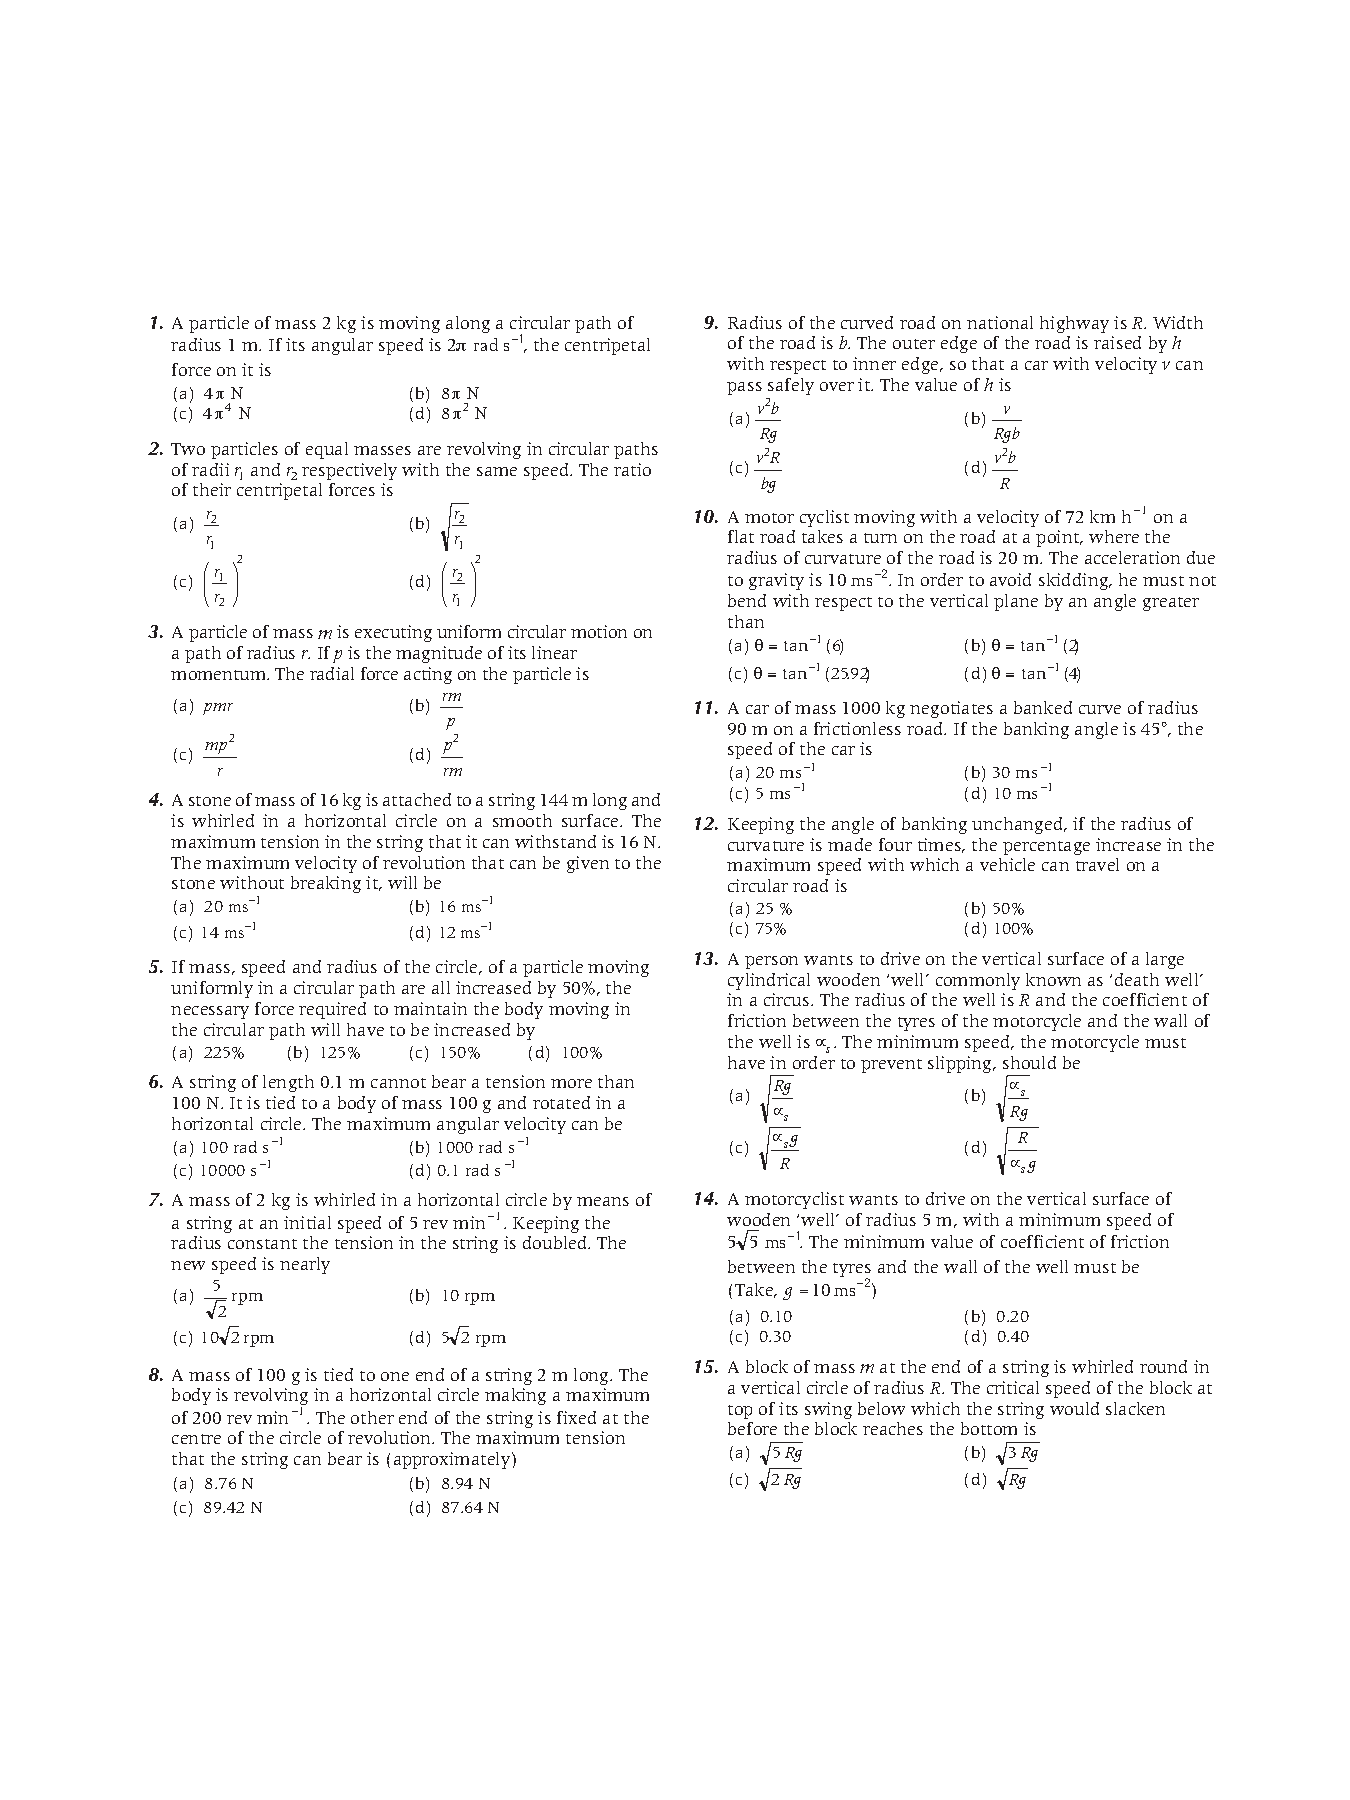
\includegraphics[trim={0 0 0 0},clip, width=170 mm]{1-15}
\linebreak
%\begin{enumerate}\addtocounter{enumi}{35}
%
%\end{enumerate}


\pagebreak
\begin{center}
\texttt{ANSWER}\\Section-B
\end{center}
\begin{enumerate}
\item (d)
\item (a)
\item (d)
\item (d)
\item (b)
\item (a)
\item (d)
\item (d)
\item (a)
\item (b)
\item (b)
\item (d)
\item (a)
\item (d)
\item (d)
\end{enumerate}


\end{document}